\documentclass[11pt,a4paper]{article}
\usepackage[utf8]{inputenc}
\usepackage[vietnamese]{babel}
\usepackage{amsmath,amssymb}
\usepackage[version=4]{mhchem}
\usepackage{geometry}
\geometry{top=1.5cm,bottom=1.2cm,left=1.4cm,right=1.4cm,headheight=28pt,headsep=12pt,footskip=18pt}
\usepackage{graphicx}
\usepackage{xcolor}
\usepackage{tabularx}
\usepackage{array}
\usepackage{colortbl}
\usepackage{tikz}
\usepackage{chemfig}
\usepackage{fancyhdr}
\usepackage{enumitem}
\usepackage{multido}
\usepackage{tcolorbox}

\definecolor{hfRed}{HTML}{D32F2F}
\definecolor{hfGreen}{HTML}{8BC390}
\definecolor{mainGreen}{HTML}{2E7D32}
\definecolor{solBlue}{HTML}{1565C0}
\definecolor{tableGreen}{HTML}{E8F5E9}

\usepackage{ex_test}

\pagestyle{fancy}
\fancyhf{}
\renewcommand{\headrulewidth}{0.75pt}
\renewcommand{\headrule}{\hbox to\headwidth{\color{hfGreen}\leaders\hrule height \headrulewidth\hfill}}
\renewcommand{\footrulewidth}{0.75pt}
\renewcommand{\footrule}{\hbox to\headwidth{\color{hfGreen}\leaders\hrule height \footrulewidth\hfill}}

\fancyhead[L]{\small\itshape\color{hfRed}Tài liệu lưu hành nội bộ}
\fancyhead[R]{\small\color{hfRed}Thầy \textbf{TRẦN VĂN THẠNH} - 0777.470.803}

\fancyfoot[L]{\footnotesize\itshape\color{hfRed}CS1: 6/15 Nguyễn Hoàng, P. Kim Long, TP Huế \quad|\quad CS2: 24 Đặng Thái Thân, TP Huế}
\fancyfoot[R]{\small\textbf{\color{hfRed}Trang \thepage}}

\setlength{\parindent}{0pt}
\setlength{\parskip}{2pt}

\begin{document}

\begin{minipage}[t]{0.48\textwidth}
\textbf{SỞ GD\&ĐT THÀNH PHỐ HUẾ}\\
\textbf{TRƯỜNG THPT NGUYỄN CHÍ THANH}\\
\textit{ĐỀ CHÍNH THỨC}\\
\textit{(Đề thi có 04 trang)}
\end{minipage}
\hfill
\begin{minipage}[t]{0.48\textwidth}
\raggedleft
\textbf{\color{hfRed}ĐỀ KIỂM TRA CUỐI HỌC KÌ 1}\\
\textbf{NĂM HỌC 2025 -- 2026}\\
\textbf{MÔN: HÓA HỌC - LỚP 11}\\
\textit{Thời gian làm bài: 45 phút (không kể thời gian phát đề)}\\
\textbf{MÃ ĐỀ: 1101}
\end{minipage}

\vspace{4pt}
\noindent
\textit{Họ và tên:} \dotfill \textit{Số báo danh:} \dotfill

\vspace{3pt}
\noindent
\textit{\footnotesize Cho biết nguyên tử khối của các nguyên tố: $\ce{Cu} = 64; \ce{H} = 1; \ce{O} = 16; \ce{N} = 14; \ce{Fe} = 56; \ce{Al} = 27; \ce{S} = 32; \ce{C} = 12; \ce{Ba} = 137$.}

\vspace{3pt}
\hrule color{hfGreen} height 0.5pt

\vspace{6pt}
{\large\bfseries\color{mainGreen} A. PHẦN TRẮC NGHIỆM}

\vspace{3pt}
{\bfseries\color{mainGreen} PHẦN 1: TRẮC NGHIỆM NHIỀU LỰA CHỌN (16 câu -- 4 điểm)}
\textit{Thí sinh trả lời câu hỏi từ câu 1 đến câu 16, mỗi câu hỏi thí sinh chỉ chọn một phương án.}
\vspace{4pt}
\begin{ex}
Cho cân bằng hóa học: $\ce{N2(g) + 3H2(g) <=> 2NH3(g)}\quad \Delta_r H = -92\text{ kJ}$
Cân bằng trên chuyển dịch theo chiều thuận khi
\choice
{tăng nhiệt độ của hệ phản ứng.}
{thêm chất xúc tác vào hệ phản ứng.}
{tăng nồng độ $\ce{NH3}$.}
{tăng áp suất của hệ phản ứng.}
\loigiai{}
\end{ex}
\begin{ex}
Hỗn hợp X gồm các alkane: pentane ($t_s = 36{,}1^\circ\text{C}$), heptane ($t_s = 98{,}4^\circ\text{C}$), octane ($t_s = 125{,}7^\circ\text{C}$) và nonane ($t_s = 150{,}8^\circ\text{C}$). Có thể tách riêng các chất đó một cách thuận lợi bằng phương pháp nào sau đây?
\choice
{Chưng cất.}
{Chiết.}
{Kết tinh.}
{Sắc kí.}
\loigiai{}
\end{ex}
\begin{ex}
Để tạo độ xốp cho một số loại bánh, có thể dùng chất nào sau đây?
\choice
{\ce{NaCl}.}
{\ce{(NH4)3PO4}.}
{\ce{CaCO3}.}
{\ce{NH4HCO3}.}
\loigiai{}
\end{ex}
\begin{ex}
Sulfur là chất oxi hóa trong phản ứng nào sau đây?
\choice
{$\ce{S + 3F2 -> SF6}$}
{$\ce{S + O2 ->[t^\circ] SO2}$}
{$\ce{S + Fe ->[t^\circ] FeS}$}
{$\ce{S + 2H2SO4 ->[t^\circ] 3SO2 + 2H2O}$}
\loigiai{}
\end{ex}
\begin{ex}
Nhóm chức là
\choice
{Là một nguyên tử bất kì trong phân tử chất hữu cơ}
{Là một nguyên tử (hoặc nhóm nguyên tử) gây ra những phản ứng hoá học đặc trưng của phân tử hợp chất hữu cơ}
{Là một nhóm nguyên tử khác biệt trong chất hữu cơ}
{Là một nhóm nguyên tử có cấu trúc không gian đặc biệt mà trong đó các nguyên tử liên kết với nhau không theo quy tắc hoá trị nào}
\loigiai{}
\end{ex}
\begin{ex}
Chất nào sau đây là chất điện li?
\choice
{saccharose}
{sulfuric acid}
{glucose}
{ethyl alcohol}
\loigiai{}
\end{ex}
\begin{ex}
Hợp chất X có công thức khung phân tử như sau:
\begin{center}
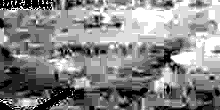
\includegraphics[width=0.25\textwidth]{images_nguyenchithanh_ma1101/khung_c7_clean.png}
\end{center}
Tổng số nguyên tử hydrogen trong X là
\choice
{10}
{12}
{6}
{8}
\loigiai{}
\end{ex}
\begin{ex}
Cho iron (III) oxide tác dụng với nitric acid loãng thì sản phẩm thu được là
\choice
{$\ce{Fe(NO3)3}, \ce{NO2}$ và $\ce{H2O}$.}
{$\ce{Fe(NO3)3}$ và $\ce{H2O}$.}
{$\ce{Fe(NO3)3}, \ce{NO}$ và $\ce{H2O}$.}
{$\ce{Fe(NO3)3}, \ce{N2}$ và $\ce{H2O}$.}
\loigiai{}
\end{ex}
\begin{ex}
Hợp chất X tan trong nước tạo dung dịch không màu. Dung dịch này không tạo kết tủa với dung dịch $\ce{BaCl2}$, khi phản ứng với $\ce{NaOH}$ tạo ra khí mùi khai, khi phản ứng với dung dịch $\ce{HCl}$ tạo ra khí làm đục nước vôi trong và làm mất màu dung dịch nước bromine. Chất X là
\choice
{\ce{(NH4)2SO3}}
{\ce{(NH4)2CO3}}
{\ce{NH4HCO3}}
{\ce{NH4HSO3}}
\loigiai{}
\end{ex}
\begin{ex}
Chất nào dưới đây là đồng đẳng của ethanol $\ce{CH3CH2OH}$?
\choice
{$\ce{CH3OCH2CH3}$.}
{$\ce{CH2=CHCH2OH}$.}
{$\ce{CH3OCH3}$}
{$\ce{CH3CH2CH2CH2OH}$.}
\loigiai{}
\end{ex}
\begin{ex}
Một số cơ sở sản xuất thuốc Bắc thường đốt một chất bột rắn X màu vàng (là một đơn chất) để tạo ra khí Y nhằm mục đích tẩy trắng, chống mốc. Tuy nhiên, theo các nhà khoa học thì khí Y có ảnh hưởng không tốt đến cơ quan nội tạng và khí Y cũng là một trong những nguyên nhân gây ra “mưa acid”. Chất rắn X là
\choice
{iodine.}
{carbon.}
{sulfur.}
{phosphorus.}
\loigiai{}
\end{ex}
\begin{ex}
Dụng cụ này có thể được sử dụng để tách riêng các chất trong hỗn hợp nào dưới đây?
\begin{center}
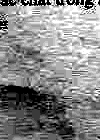
\includegraphics[width=0.15\textwidth]{images_nguyenchithanh_ma1101/pheu_chiet_c12_clean.png}
\end{center}
\choice
{Xăng và dầu ăn.}
{Nước và rượu.}
{Nước và muối ăn.}
{Dầu ăn và nước.}
\loigiai{}
\end{ex}
\begin{ex}
Chất nào sau đây không thuộc loại chất hữu cơ?
\choice
{\ce{CH3COONa}}
{\ce{Al4C3}}
{\ce{CH3Cl}}
{\ce{CCl4}}
\loigiai{}
\end{ex}
\begin{ex}
Khí thải công nghiệp, khí thải động cơ (ô tô, xe máy ...) là nguyên nhân chủ yếu gây mưa acid. Dãy nào dưới đây gồm các chất có trong các loại khí thải này và là nguyên nhân trực tiếp gây mưa acid?
\choice
{$\ce{SO2}, \ce{CO}, \ce{NO}$.}
{$\ce{SO2}, \ce{CO}, \ce{NO2}$.}
{$\ce{NO}, \ce{NO2}, \ce{SO2}$.}
{$\ce{NO2}, \ce{CO2}, \ce{CO}$.}
\loigiai{}
\end{ex}
\begin{ex}
Khi cho saccharose ($\ce{C12H22O11}$) tác dụng với dung dịch $\ce{H2SO4}$ đặc trong cốc thủy tinh thấy có bọt khí đẩy carbon trào lên khỏi cốc. Thí nghiệm trên chứng minh được tính chất nào sau đây của $\ce{H2SO4}$ đặc?
\choice
{chỉ có tính oxi hóa mạnh.}
{tính háo nước và tính oxi hóa mạnh.}
{chỉ có tính háo nước.}
{tính háo nước và tính khử mạnh.}
\loigiai{}
\end{ex}
\begin{ex}
Kim loại nào sau đây không tác dụng với dung dịch acid $\ce{H2SO4}$ loãng nguội?
\choice
{Na}
{Zn}
{Cu}
{Al}
\loigiai{}
\end{ex}

\vspace{6pt}
{\large\bfseries\color{mainGreen} PHẦN 2: TRẮC NGHIỆM ĐÚNG -- SAI (2 câu -- 2 điểm)}

\textit{Thí sinh trả lời từ câu 1 đến câu 2. Trong mỗi ý a), b), c), d) ở mỗi câu, thí sinh chọn đúng hoặc sai.}
\vspace{4pt}
\begin{ex}
Pha 1,0 L dung dịch sulfuric acid. Sau đó lấy 10,0 mL dung dịch acid cho vào bình tam giác, thêm vài giọt dung dịch phenolphathalein. Nhỏ từ từ dung dịch $\ce{NaOH}\ 0{,}10\text{ M}$ chứa trên burette vào bình tam giác đến khi dung dịch xuất hiện màu hồng nhạt, đọc thể tích $\ce{NaOH}$ đã dùng trên burette. Lặp lại thí nghiệm 3 lần, các giá trị thể tích $\ce{NaOH}$ đọc được lần lượt là 17,9 mL; 18,0 mL; 18,1 mL.
\choiceTF
{ Khi chuẩn độ xảy ra phản ứng hoá học $\ce{H2SO4 + 2NaOH -> Na2SO4 + 2H2O}$.}
{ pH của dung dịch acid gần bằng 1,05.}
{ Để pha 1 lít dung dịch sulfuric acid trên cần hoà 19,6 ml (làm tròn đến phần chục) dung dịch $\ce{H2SO4}$ 98\% (d=1,84g/ml) vào 980,4 ml nước.}
{ Phương pháp trong thí nghiệm trên là phương pháp chuẩn độ acid-base.}
\loigiai{}
\end{ex}
\begin{ex}
Đốt cháy hoàn toàn 7,25 gam hợp chất hữu cơ X thu được 11,2 lít $\ce{CO2}$ (đktc) và 11,25 gam $\ce{H2O}$. Biết tỉ khối của X so với khí nitrogen bằng 29/14.
\choiceTF
{ Phần trăm khối lượng của nguyên tố hydrogen trong X xấp xỉ 8,62\%}
{ X có chứa 4 nguyên tử carbon.}
{ Phân tử khối của X bằng 29.}
{ Phân tử X chứa 3 loại nguyên tố là C, H, O.}
\loigiai{}
\end{ex}

\vspace{6pt}
{\large\bfseries\color{mainGreen} PHẦN 3: CÂU TRẮC NGHIỆM TRẢ LỜI NGẮN (4 câu - 1 điểm)}

\textit{Thí sinh trả lời từ câu 1 đến câu 4.}
\vspace{4pt}
\begin{ex}
Hoà tan 5,4 gam aluminium (Al) bằng acid $\ce{H2SO4}$ loãng dư sinh ra V lít khí (ở đktc). Tính V.
\par\textit{Trả lời:} \dotfill
\loigiai{}
\end{ex}
\begin{ex}
Khi cho dung dịch $\ce{HNO3}$ đặc, nóng lần lượt tác dụng với các chất sau: $\ce{Cu}, \ce{Fe2O3}, \ce{C}$, dung dịch $\ce{Ba(OH)2}$, dung dịch $\ce{Na2SO3}$. Số phản ứng mà $\ce{HNO3}$ đóng vai trò là chất oxi hóa là bao nhiêu?
\par\textit{Trả lời:} \dotfill
\loigiai{}
\end{ex}
\begin{ex}
Cho các cân bằng hoá học:
\begin{align*}
(1) &\quad \ce{N2(g) + 3H2(g) <=> 2NH3(g)} \\
(2) &\quad \ce{H2(g) + I2(g) <=> 2HI(g)} \\
(3) &\quad \ce{2SO2(g) + O2(g) <=> 2SO3(g)} \\
(4) &\quad \ce{2NO2(g) <=> N2O4(g)}
\end{align*}
Khi thay đổi áp suất có bao nhiêu cân bằng hóa học bị chuyển dịch?
\par\textit{Trả lời:} \dotfill
\loigiai{}
\end{ex}
\begin{ex}
Ứng với CTPT $\ce{C3H8O}$ có bao nhiêu đồng phân cấu tạo thuộc loại alcohol?
\par\textit{Trả lời:} \dotfill
\loigiai{}
\end{ex}

\vspace{6pt}
{\large\bfseries\color{mainGreen} B. PHẦN TỰ LUẬN (3 câu -- 3 điểm)}

\textit{Thí sinh trình bày lời giải chi tiết vào phần giấy làm bài thi.}
\vspace{4pt}
\textbf{Câu 1: (0,5 điểm)} Viết công thức cấu tạo thu gọn và công thức khung phân tử các đồng phân cấu tạo ứng với công thức phân tử $\ce{C4H10}$.

\vspace{2pt}
\multido{}{6}{\noindent\dotfill\par\vspace{2pt}}

\vspace{4pt}
\textbf{Câu 2: (1,0 điểm)} Caffeine là chất kích thích tự nhiên được tìm thấy trong cây trà, cà phê và ca cao. Chúng hoạt động bằng cách kích thích não và hệ thần kinh trung ương, giúp con người tỉnh táo và ngăn ngừa sự mệt mỏi. Thành phần phần trăm về khối lượng của các nguyên tố trong phân tử caffeine như sau: 49,48\% carbon; 5,15\% hydrogen; 28,87\% nitrogen còn lại là oxygen. Phổ MS của caffeine được cho như hình dưới đây:

\begin{center}
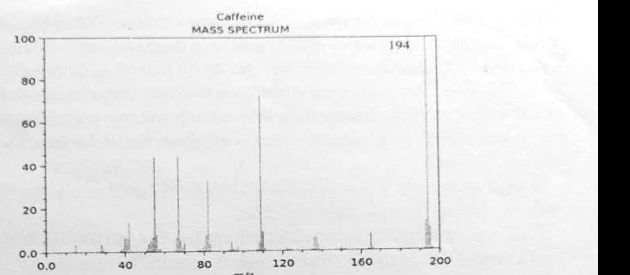
\includegraphics[width=0.7\textwidth]{images_nguyenchithanh_ma1101/ms_caffeine_clean.png}
\end{center}

a. Dựa vào phổ khối lượng phân tử (MS) hãy xác định phân tử khối của caffeine?\\
b. Xác định công thức phân tử của caffeine.

\vspace{2pt}
\multido{}{8}{\noindent\dotfill\par\vspace{2pt}}

\vspace{4pt}
\textbf{Câu 3: (1,5 điểm)} Sulfuric acid là một trong những hoá chất quan trọng nhất được sử dụng trong công nghiệp; được sản xuất hàng trăm triệu tấn mỗi năm, chiếm nhiều nhất trong ngành công nghiệp hoá chất. Sulfuric acid được sản xuất từ quặng pyrite theo sơ đồ sau:
\[
\ce{FeS2 ->[(1)] SO2 ->[(2)] SO3 ->[(3)] oleum ->[(4)] H2SO4}
\]
a. Hoàn thành sơ đồ phản ứng trên, ghi rõ điều kiện phản ứng nếu có.\\
b. Hấp thụ toàn bộ lượng $\ce{SO3}$ điều chế được từ $m\text{ kg } \ce{FeS2}$ vào 1000 gam dung dịch $\ce{H2SO4}\ 98\%$ thu được oleum X. Hoà tan 50,7 gam X vào nước được dung dịch Y. Cho dung dịch $\ce{BaCl2}$ dư vào Y thu được 139,8 gam kết tủa. Giả sử các phản ứng xảy ra hoàn toàn. Tìm $m$.

\vspace{2pt}
\multido{}{12}{\noindent\dotfill\par\vspace{2pt}}

\vspace{6pt}
\begin{center}
\textbf{\large ---------- HẾT ----------}
\end{center}

\end{document}
